\subsection{Anfälligkeit der ungeschützten Modelle}
Der Robustifizierungsprozess eines Modells ist sehr zeitintensiv. Daher wurde entschieden, für die erfolgreich trainierten Modellklassen DenseNet, EfficientNetV2 und ResNet ein kleines und ein mittelgrosses Modell auf beiden Datensätzen anzugreifen und zu robustifizieren. Hier wird die Anfälligkeit der Modelle gegenüber \acrshort{uap}s vor jeglicher \Gls{robustifizierung} analysiert.

\subsubsection{AUROC Metriken}
Beim Vergleich der AUROC-Modellmetriken in Abbildung \ref{fig:auroc-uap} wird sichtbar, dass sowohl die Validierungs- als auch die Testmetriken bei eingefügten \acrshort{uap}s sinken. Ausnahmen bilden das ResNet50 und das EfficientNetV2-M Modell auf dem COVIDx CXR-4 Datensatz, welche bei den Testmetriken sogar eine Verbesserung aufweisen. Da diese Metriken jedoch bereits sehr niedrig sind und das $\approx$ 68\%-Konfidenzintervall (1$\sigma$) den Wert ohne \acrshort{uap}s umfasst, werden diese Werte als nicht aussagekräftig genug beachtet.

\begin{figure}[H]
    \centering
    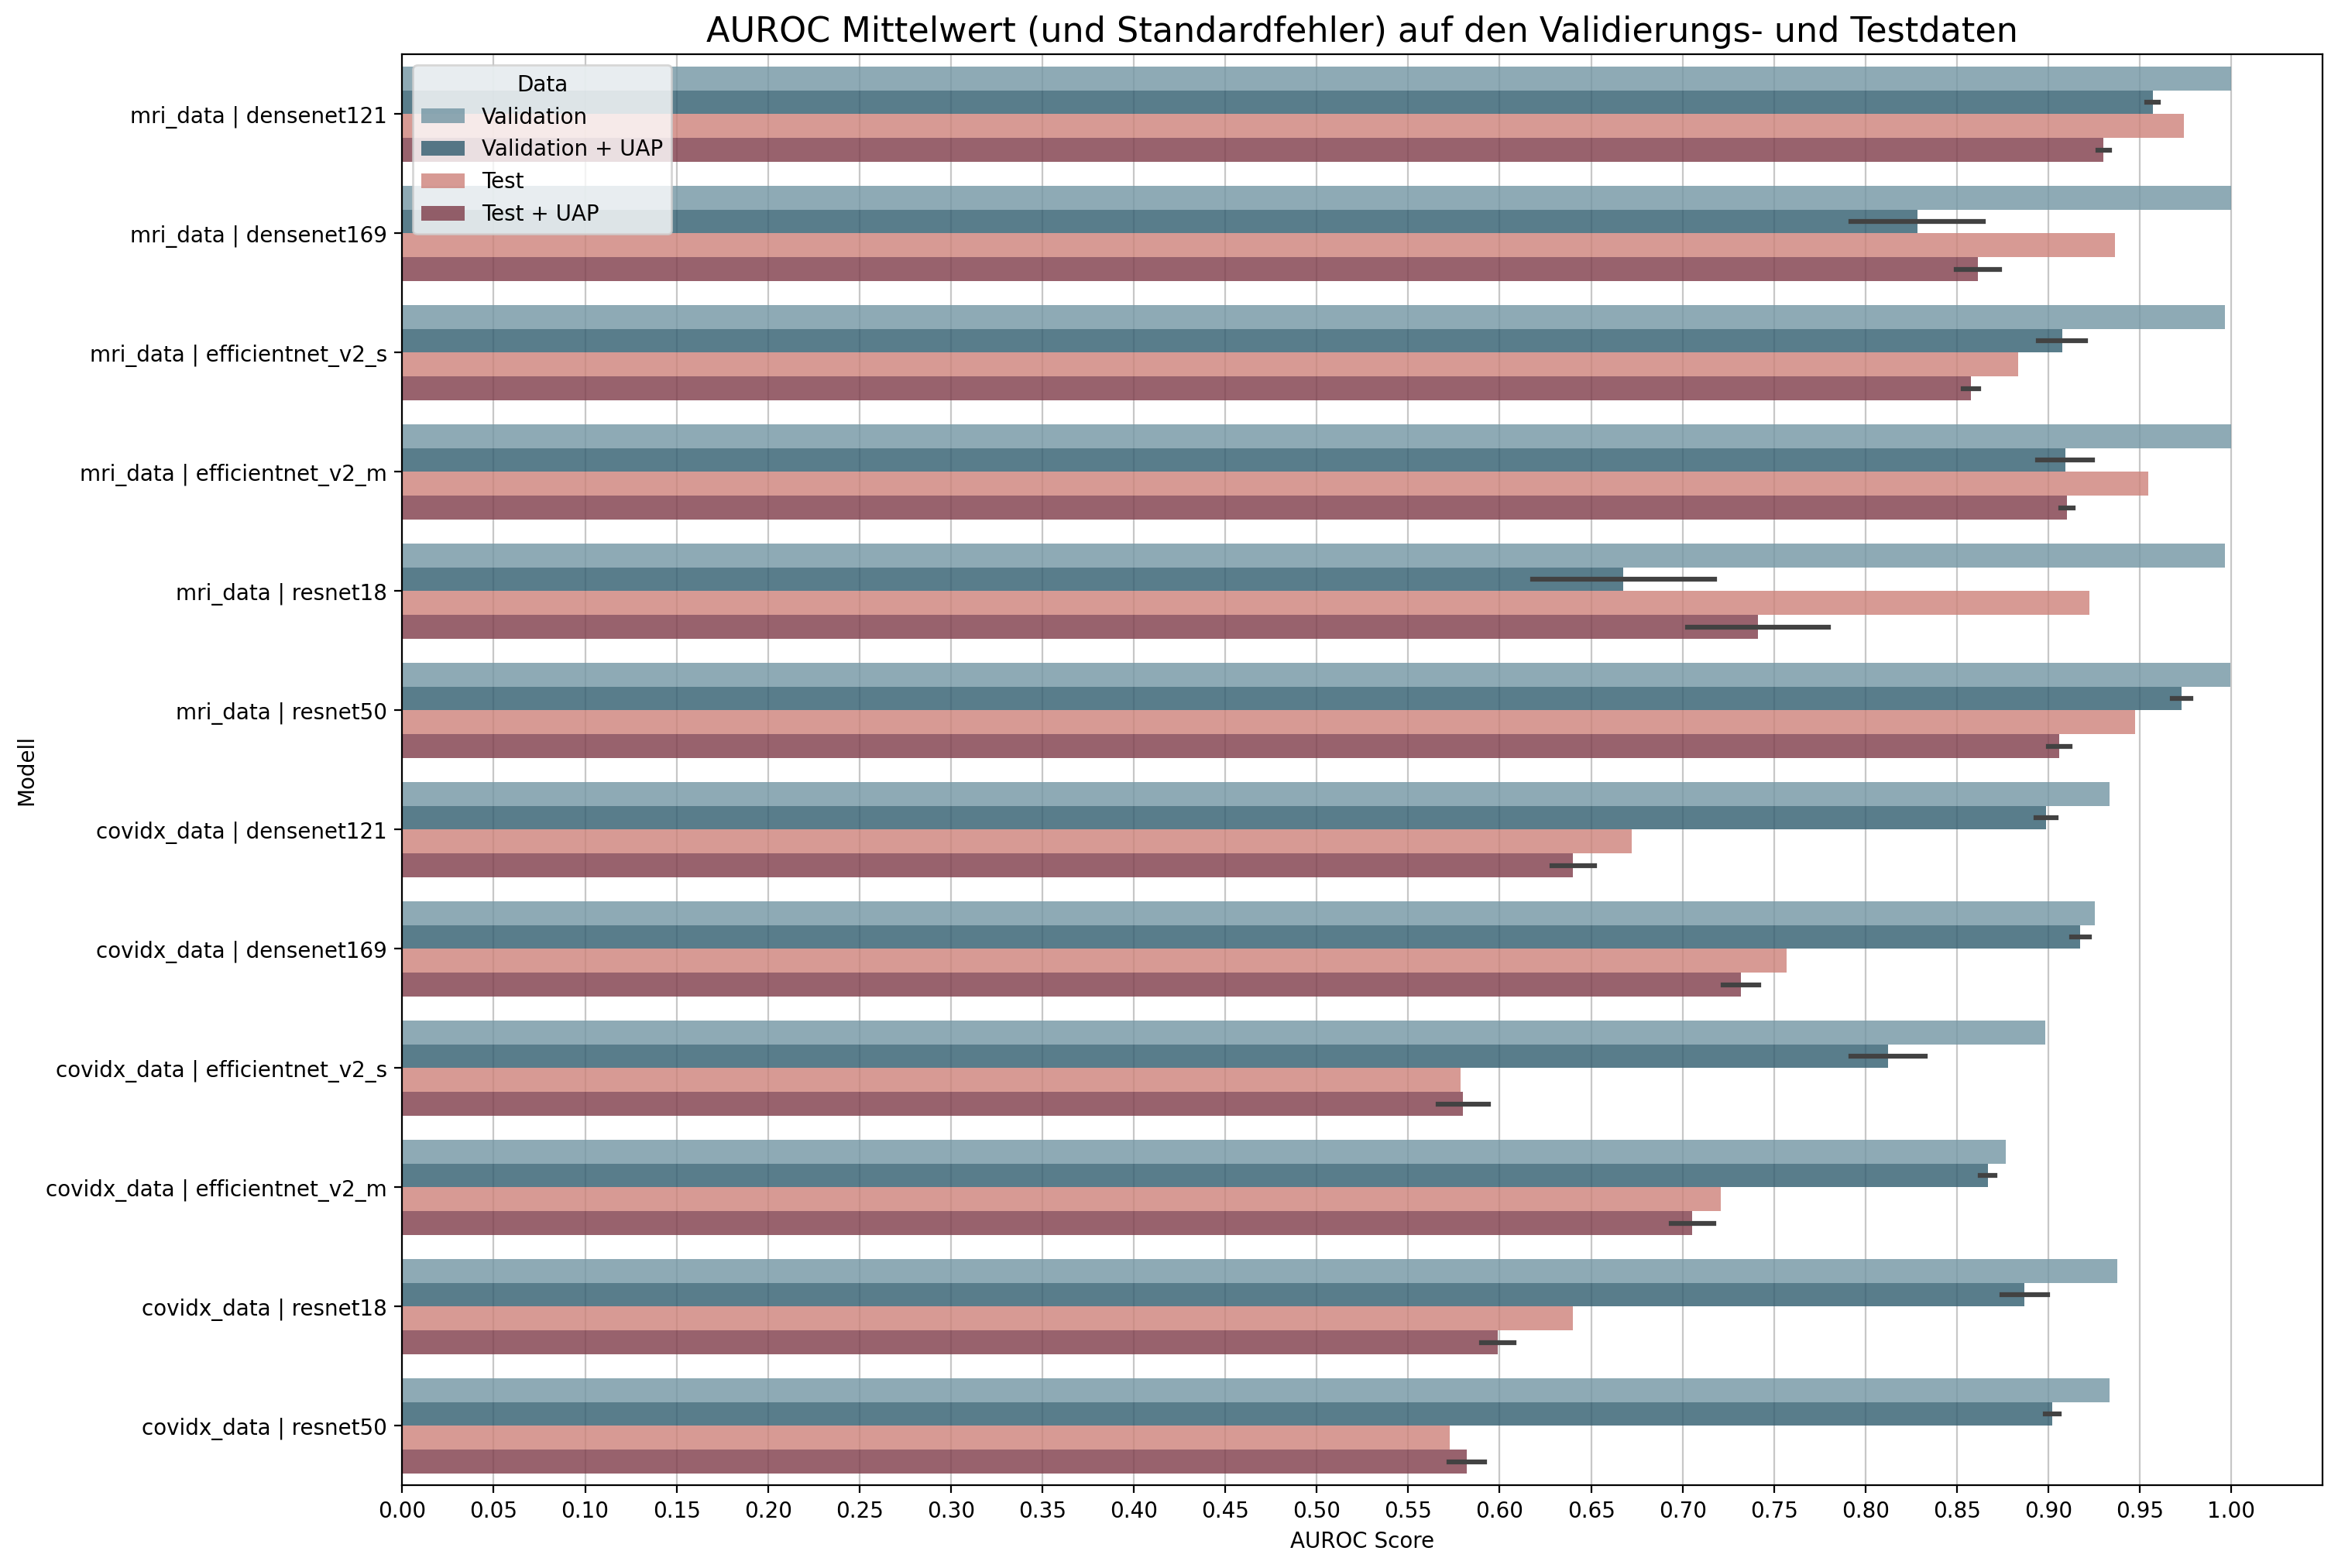
\includegraphics[width=\linewidth]{01-images/05-resultate/AUROCScores_UAP.png}
    \caption{AUROC Metriken der Modelle mit und ohne UAPs}
    \label{fig:auroc-uap}
\end{figure}

\newpage

\subsubsection{Recall Metriken}
Da der Perturbationsalgorithmus darauf ausgelegt ist Falsch-Negativ Klassifikationen zu verursachen, ist es sinnvoll, auch die Recall-Metrik in Abbildung \ref{fig:recall-uap} zu betrachten. Dabei zeigen sich grössere Differenzen im Vergleich zu den AUROC-Metriken. Bei jedem Modell nimmt die Recall-Metrik mit der Addition der \acrshort{uap}s signifikant ab. Durch die Anpassung der Mindesttäuschungsrate $r$ und des Regularisierungsparameters der Matrizennorm $\lambda_{norm}$ bei der Generierung der \acrshort{uap}s können diese Differenzen sogar vergrössert werden.

\begin{figure}[H]
    \centering
    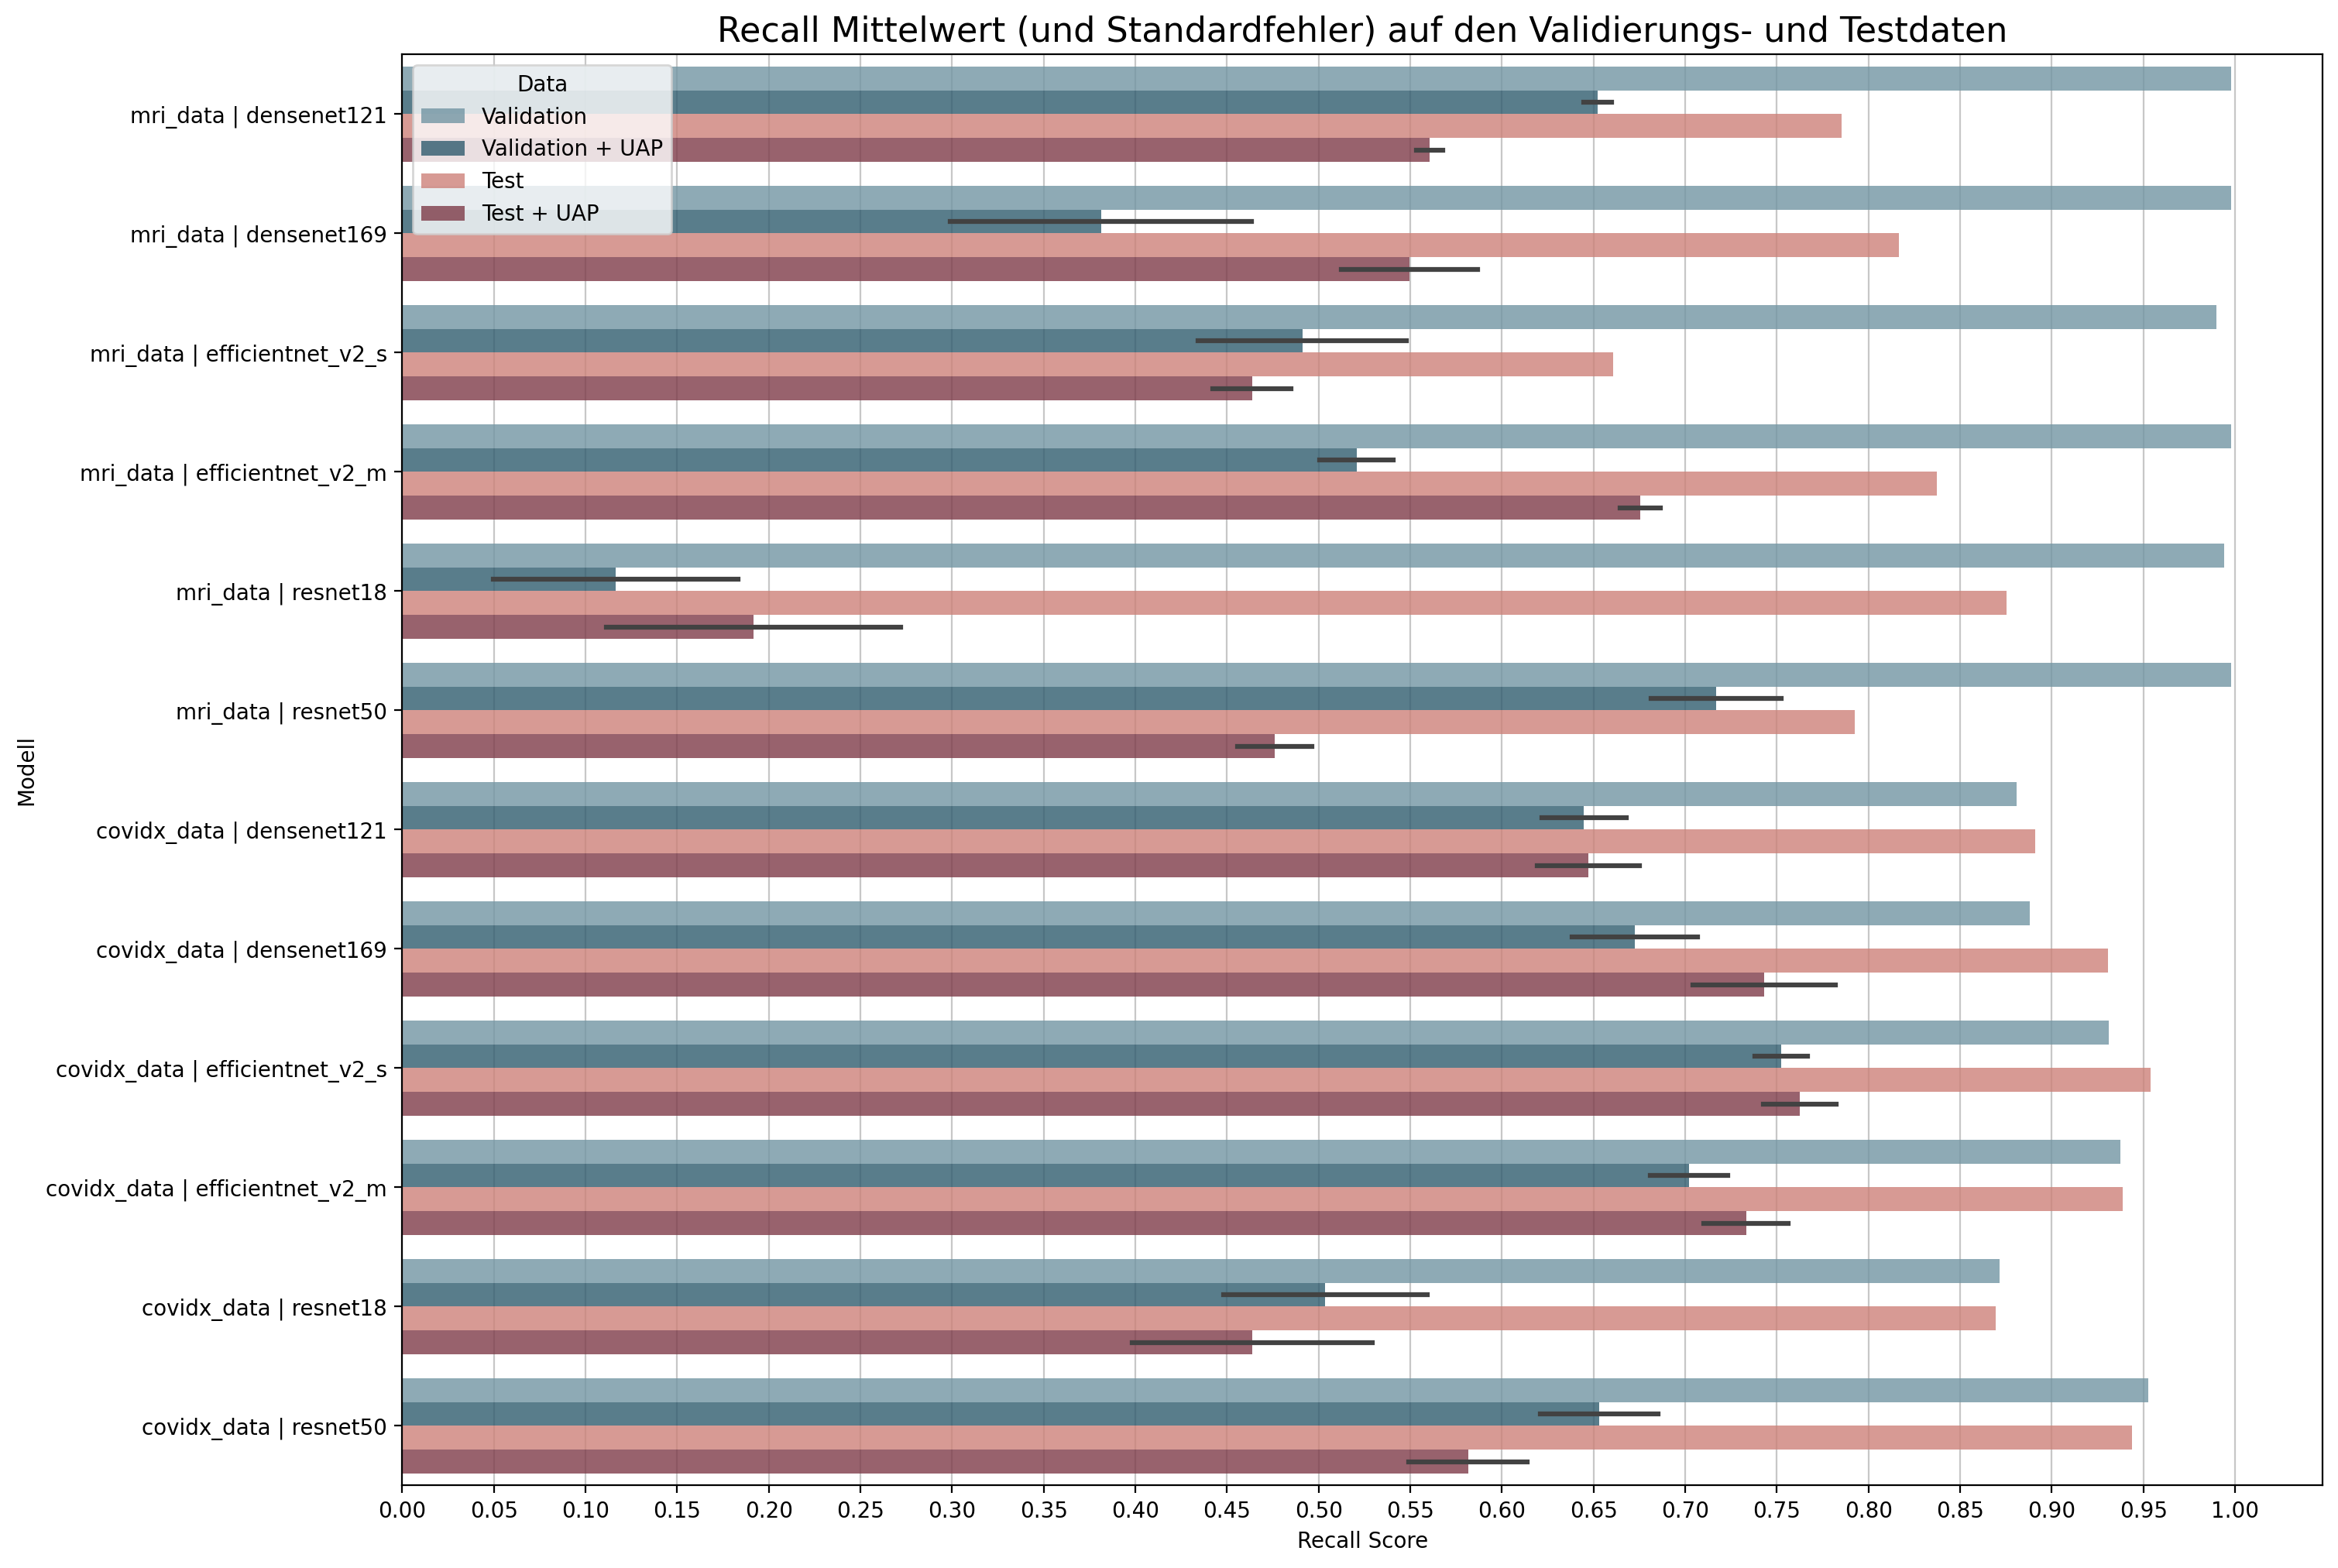
\includegraphics[width=\linewidth]{01-images/05-resultate/RECALLScores_UAP.png}
    \caption{Recall Metriken der Modelle mit und ohne UAPs}
    \label{fig:recall-uap}
\end{figure}

Aus dieser Analyse lässt sich erschliessen, dass die ungeschützten Modelle sehr anfällig gegenüber den generierten \acrshort{uap}s sind und dass der angepasste Algorithmus erfolgreich Perturbationen generieren kann, welche zu Falsch-Negativ Klassifikationen führen.
